\section{PID pozíció szabályozás szimmetrikus optimum módszerrel}

%{{{ P, I és D paraméterek számítása
\subsection{P, I és D paraméterek számítása}

Az előző feladatból a szabályzót változtassuk meg egy PID kontrollerre.

Írjuk fel az előrevezető ág átviteli függvényét:
\begin{equation}
	\fn{W}_\text{x} = \fn{W}_\text{c}\fn{W}_\text{x}\frac{1}{s} = 
	\frac{A\, P\, \left(T_\text{I}\, s + 1\right)}{T_\text{I}\, s^2\, \left(T_1\, s + 1\right)\, \left(T_2\, s + 1\right)},
	\frac{A\, P\, \left(\frac{1}{T_\text{I}\, s} + \frac{T_\text{D}\, s}{n\,T_\text{D}\, s + 1} + 1\right)}{s\, \left(T_1\, s + 1\right)\, \left(T_2\, s + 1\right)}
\end{equation}
ahol $A$ a szabályozott szakasz erősítése.

Ezután írjuk fel a fázistolást a körfrekvencia függvényében:
\begin{equation}
	\varphi(\omega) = -\pi - \operatorname{arctg}(T_1\omega) - \operatorname{arctg}(T_2\omega) + \operatorname{arctg}(T_\text{I}\omega).
\end{equation}
Ennek a függvénynek a szélsőértékét keressük. Ehhez tegyük nullává a deriváltat:
\begin{equation}
	\frac{\partial\varphi}{\partial\omega} = 
	\frac{T_\text{I}}{T_\text{I}^2\, \omega^2 + 1} - \frac{T_2}{{T_2}^2\, \omega^2 + 1} - \frac{T_1}{{T_1}^2\, \omega^2 + 1} = 0.
\end{equation}
Ebből megkaptunk egy $\omega_\text{c}$ értéket, ami $T_\text{I}$-től függ.
Ezt helyettesítsük be a fázistartalékhoz tartozó képletbe, ami kiadja $T_\text{I}$-t és
ezáltal $\omega_\text{c}$ numerikus értékét is:
\begin{equation}
	\varphi_\text{t} = \pi + \varphi(\omega_\text{c}) \Rightarrow T_\text{I}.
\end{equation}
Ebből $T_\text{I} = 0,204$ s, és $\omega_\text{c} = 18,2783~\frac{\text{rad}}{\text{s}}$.

Már csak a $P$ körerősítést kell meghatároznunk, ami ugyanúgy történik mint az első feladatban:
\begin{equation}
	\abs{\fn{W}_\text{x}(\omega_\text{c})} = 1 \Rightarrow P = 1,0642.
\end{equation}

Ellenőrizzük, hogy a fázistartalék tényleg $60^\circ$-e a \verb|margin| függvénnyel.
\begin{figure}[H]
	\centering
	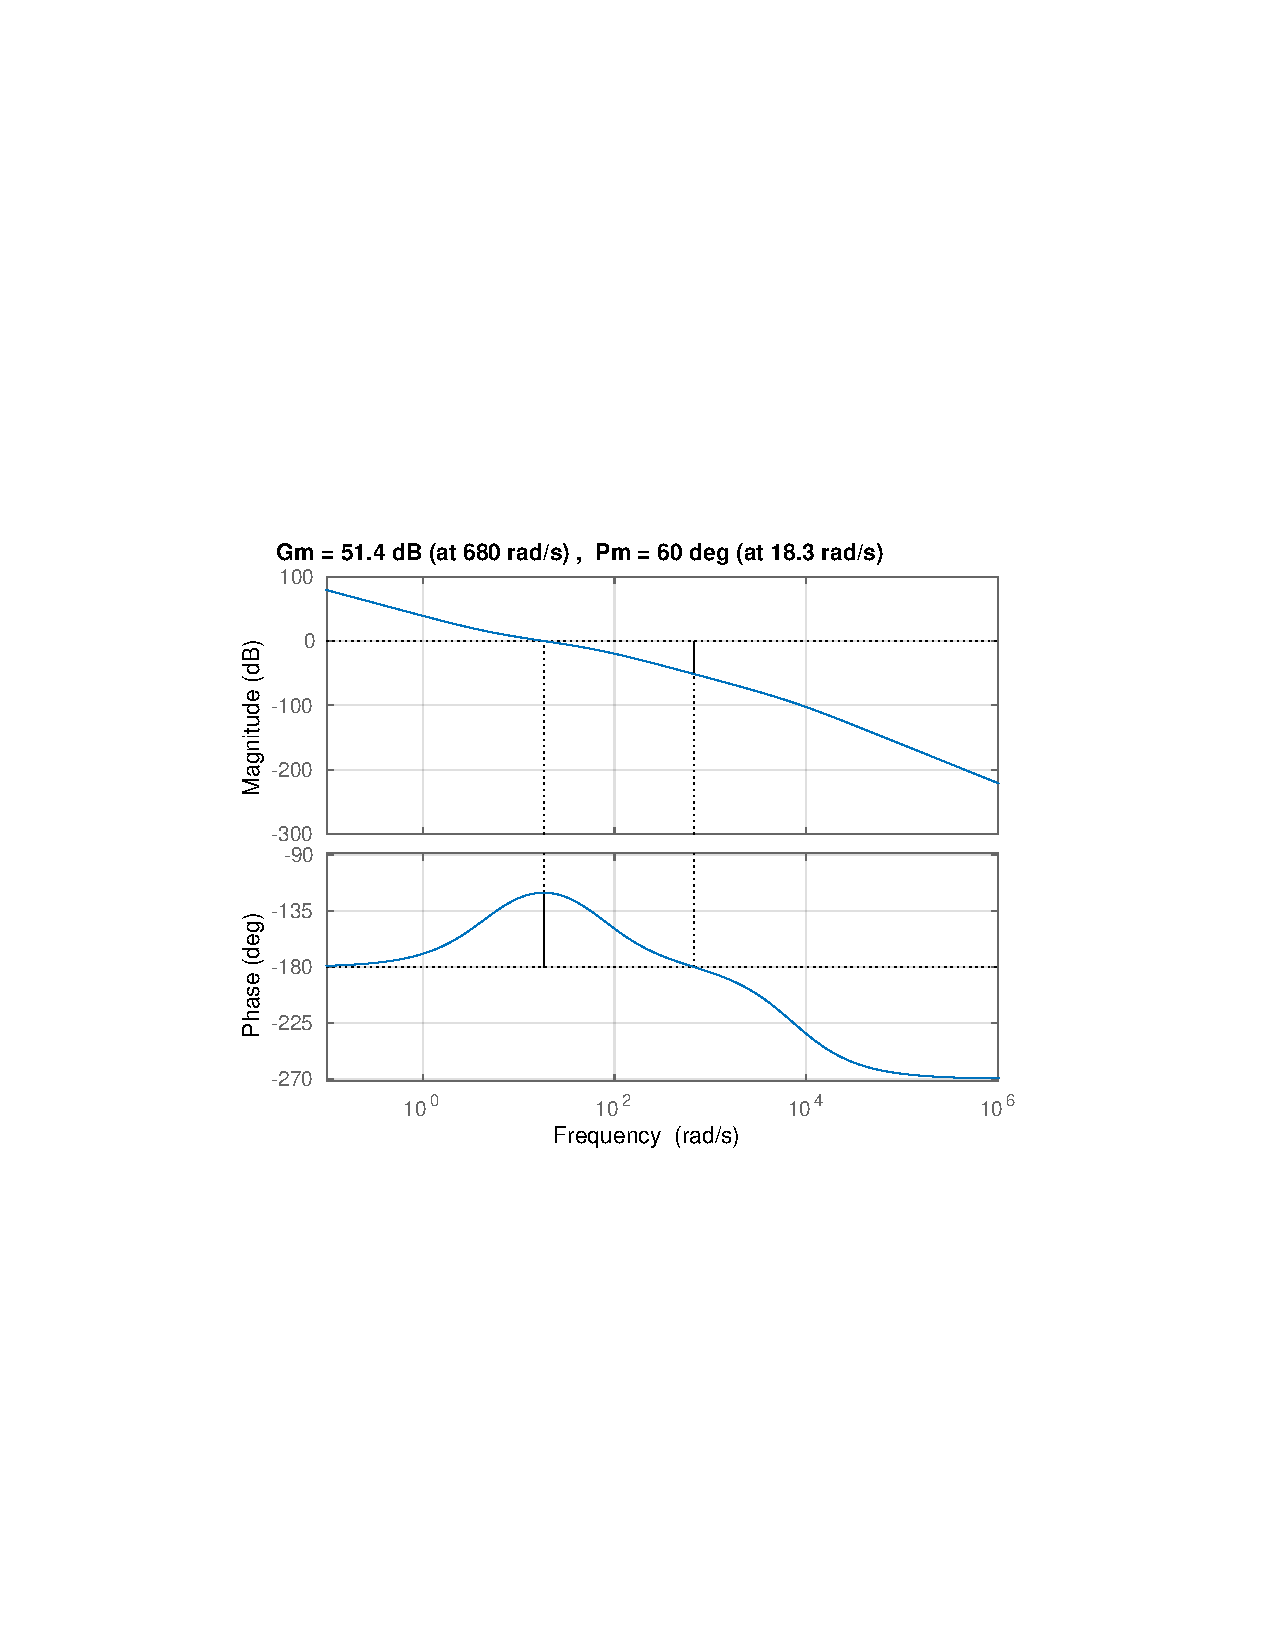
\includegraphics[width=.7\textwidth, trim=100 240 80 252, clip]{3a_margin}
	\caption{Pozíció-szabályzott rendszer Bode-diagramja, fázistartalék feltüntetve}
	\label{fig:3a_margin}
\end{figure}

Ez teljesül.

%}}}

%{{{ Egységugrás válasz
\subsection{Egységugrás válasz}

Egy kör fordulat szabályozása esetén a bemenet Laplace-transzformáltja $\fn{X}=\frac{2\pi}{s}$,
a kimenet ebből $\fn{Y} = \fn{W}_\text{cl}\fn{X}$. Ezt a szokásos \verb|step| függvény
ki is rajzolja nekünk időtartományban, amit \aref{fig:3b_step}. ábra mutat.

\begin{figure}[H]
	\centering
	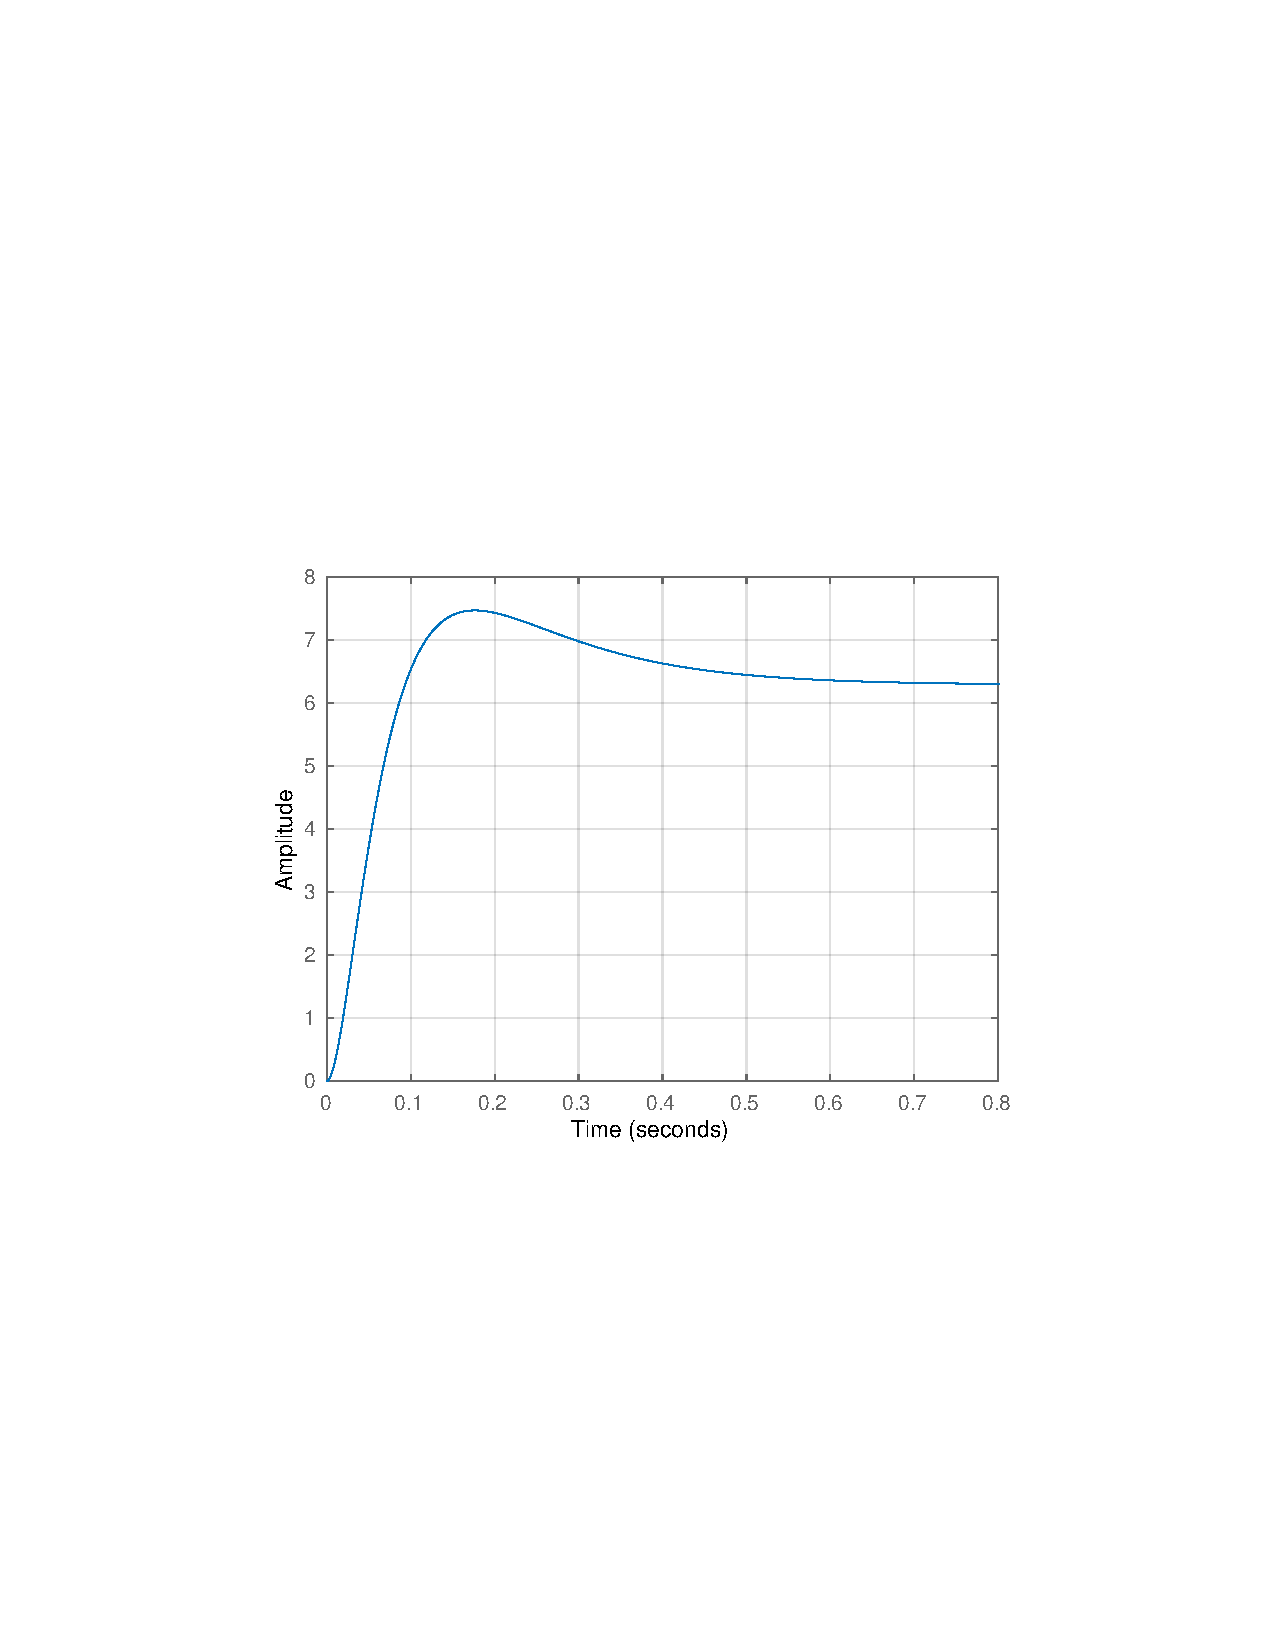
\includegraphics[width=.7\textwidth, trim=100 240 80 252, clip]{3b_step}
	\caption{PI egységugrás-válasz}
	\label{fig:3b_step}
\end{figure}

%}}}

%{{{ Állandósult szögsebesség
\subsection{Állandósult szögsebesség}

Az előző részfeladatban kiszámolt kimenetet felhasználva az állandósult szög érték:
$\omega_\infty = \lim\limits_{s\rightarrow 0}s\fn{Y} = 6,2832^\circ$.

Az állandósult hiba a PI szabályzótól vártan zérus.

%}}}
